\section{Pyrocumulonimbus}
  \label{pcb}
  
  Pyrocumulonimbus (PCB) is the phenomenon whereby a large thunderstorm system is generated by the heat and moisture entrained and lofted by a fire.
  These are extremely dangerous, difficult to predict, drastically change local weather, and can lead to substantial spotting and lightning \cite{Peace2017}.
  
  \paragraph{PCB Formation} is driven by the massive amounts of heat energy output from fires, which can be entrained in large scale updrafts.
  When a fire spreads fast is when the most heat is being produced, which is when the risk of PCB formation is greatest.
  Near-surface atmospheric stability and dynamics affects both how the heat entrains into the atmosphere and how fast the fire spreads.
  This means that simulated PCB are quite sensitive to the sorts of atmospheric parameters that affect horizontal and vertical movement, and near-surface stability.
  TODO: Some stuff about vorticity and other metrics?
  
  \paragraph{PCB Formation Threshold (PFT)}
  Kevin's PFT - TODO: point to his publication.
  Weather conditions can be more or less suitable for PCB generation, one way of quantifying this is through the PFT that estimates how much energy needs to be released by a fire to create a PCB.
  The less energy required, the more likely we are to see PCB formation.
  PFT calculations can be heavily influenced by energy in the system coming from the coupled fire model, making PFT analysis unsuitable downwind of the fire.
  Analysis on PFT in this work therefor either uses PFT calculated somewhere upwind of the fire, or meteorological output from an uncoupled (but otherwise identical) model run.
  
  \subsection{Waroona}
    \label{pcb:waroona}
    
    PFT from code developed by Kevin Tory can tell us whether PCB formation is likely.
    Fire output is compared to PFT calculated just upwind of the fire ignition point in figure \ref{fig:pcb:waroona:PFT}.
    Fire power at several times exceeds the PFT, and we might expect to see PCB within the model output.
    This is not a sure thing as PFT calculations can vary greatly over a small distance, and upwind conditions may not represent those at the firefront.
    
    \begin{figure}
      \includegraphics[width=\linewidth]{../../figures/waroona_run3/PFT_work/comparison/firepower.png}
      \caption{%
        Fire power output, and PFT calculated approximately 1~km upwind from the fire ignition for the Waroona fire simulation.
      }
      \label{fig:pcb:waroona:PFT}
    \end{figure}
    
    
    Strong cylindrical upward motion and cloud formation over the fire front can be considered clear evidence of PCB.
    To home in on where PCB occur, I zoom to a subset of the horizontal region that surrounds the fire. Horizontal model slices (at varying altitudes) of vertical wind motion and total cloud content show wind and cloud structures above the fire zone (Figure \ref{fig:pcb:waroona:vert_motion_slices}).
    A clear cylindrical plume occurs from around 5~km altitude all the way up to the stratosphere ($\sim 15$~km).
    Cross sections show a strong internal updraft surrounded by downdrafts throughout the troposphere (Figure \ref{fig:pcb:waroona:pcb_transects}).
    

    \begin{figure}
      \includegraphics[width=\linewidth]{../../figures/waroona_run3/vert_motion_slices/fig_201601060630.png}
      \caption{%
        Top-down views of vertical motion on model levels of increasing altitude from left to right, top to bottom. 
        Grey dots represent Waroona, and Yarloop (north, south respectively), with a blue star showing a weather station site.
        A red contour shows the fire front, and cloud content above the 0.1 g\/kg threshold is marked by stippling.
        }
      \label{fig:pcb:waroona:vert_motion_slices}
    \end{figure}
    
    \begin{figure}
      \includegraphics[width=\linewidth,height=\textheight]{../../figures/waroona_run3/pyrocb/fig_201601060630.png}
      \caption{%
        Top panel: top-down view showing the firefront (red contour) and vertical motion near Waroona.
        Bottom panels: transects (over dashed lines in Top panel) showing vertical motion, cloud content (black contour on 0.1 g\/kg ice and water content) and winds.
      }
      \label{fig:pcb:waroona:pcb_transects}
    \end{figure}

    Visualisation in three dimensions gives a much clearer view of the PCB formation and scale. 
    Figure \ref{fig:pcb:waroona:pcb_3d} shows the PCB on model levels, with heat, vertical motion, and topography represented at roughly the time of formation and the peak of the storm activity.
    The front produces enough heat to form a huge plume that punches up into the upper troposphere, entraining moisture and leading to very strong mixing and winds locally.

    \begin{figure}
      \centering
      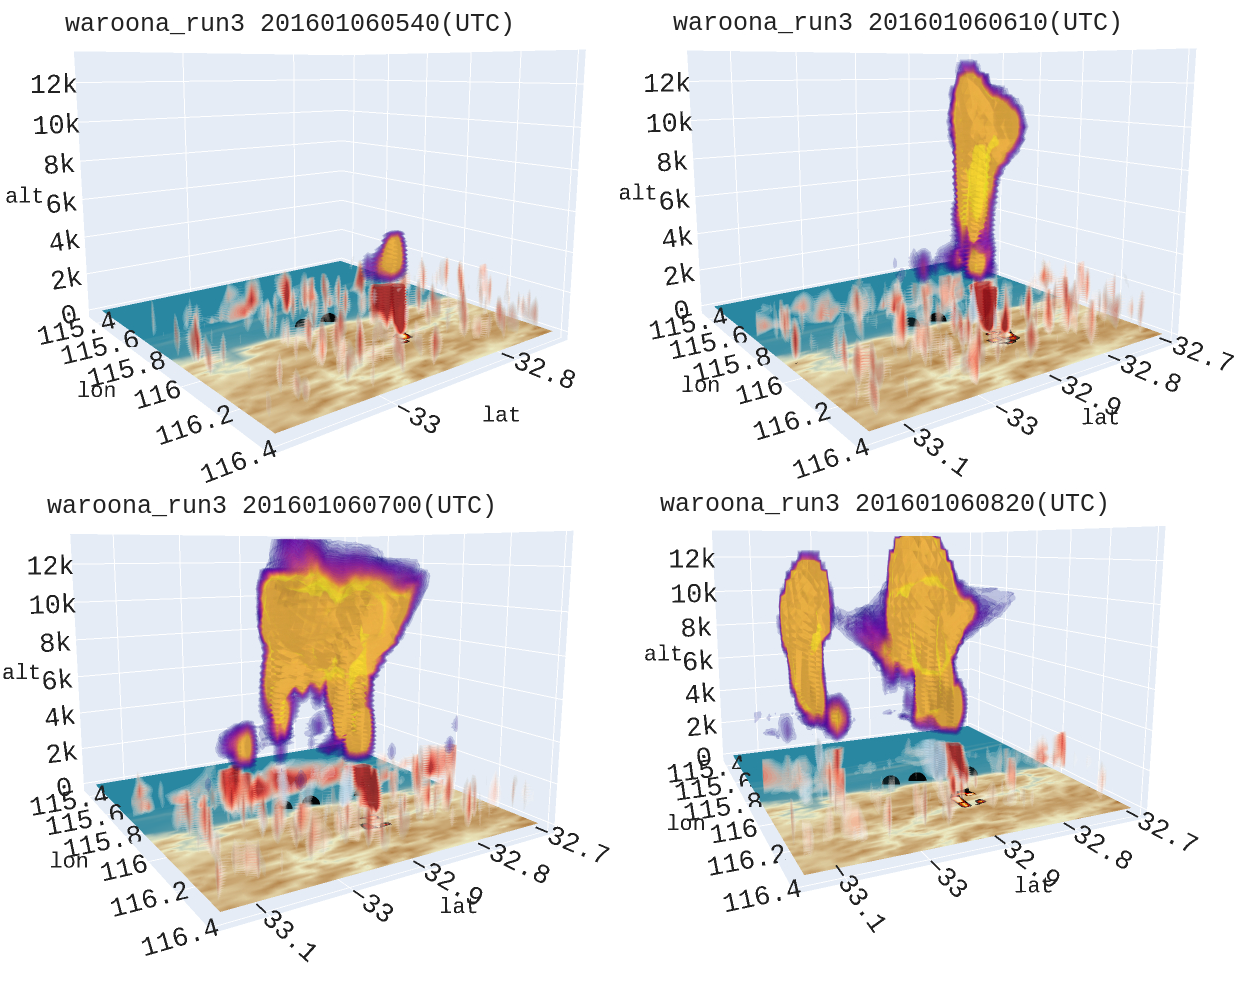
\includegraphics[width=1\linewidth]{../../figures/project/threedee/waroona_run3_pcb.png}
      \caption{%
        Three dimensional representation of meteorology near the fire over Waroona, at four times (one time per panels), with x, y, and z dimensions being longitude, latitude, and altitude above ground level respectively.
        Purple to yellow volumes show cloud content (0.1 g\/kg threshold).
        Red and blue volumes show vertical motion between 3-6 m\/s up to 2~km altitude above ground level.
        Near the surface a black-red-yellow volume may be visible if potential temperature is greater than 311~K, this shows where the fire is releasing the most heat.
        Altitude zero shows a teal to brown filled contour surface coloured by ground level altitude.
        }
      \label{fig:pcb:waroona:pcb_3d}
    \end{figure}

  
  \subsection{Sir Ivan}
    \label{pcb:sirivan}
    
    The simulation over Sir Ivan showed that weather was generally unfavourable to PCB formation until about 3PM, when the PFT dropped by a couple of orders of magnitude (Fig \ref{fig:pcb:sirivan:pft_series}).
    The Sir Ivan fire covered a large area, and the conditions upwind of the fire ignition are not fully representative of those near the fire front, and from other model output we see that a PCB occurs at around 5PM lasting on the order of an hour.
    Figure \ref{fig:pcb:sirivan:pcb_transects} shows the location and dynamics of the PCB, which stretched up to the top of the troposphere, driving turbulent wind conditions and cloud formation locally.
    
    \begin{figure}
      \centering
      \includegraphics[width=1\linewidth]{../../figures/sirivan_run1/PFT_work/comparison/firepower}
      \caption{%
        Time series for 24 hours of simulation firepower and PFT.
        PFT calculated for a vertical column approximately 1~km upwind of the fir ignition.
        }
      \label{fig:pcb:sirivan:pft_series}
    \end{figure}


    \begin{figure}
      \centering
      \includegraphics[width=1\linewidth]{../../figures/sirivan_run1/pyrocb/fig_201702120701.png}
      \caption{%
        Top panel: top-down view showing the firefront (red contour) and vertical motion near Sir Ivan.
        Bottom panels: transects (over dashed lines in Top panel) showing vertical motion, cloud content (black contour on 0.1 g\/kg ice and water content), and winds.
        }
      \label{fig:pcb:sirivan:pcb_transects}
    \end{figure}
    
    Sir is at higher altitude, and latitude, and had a larger burn area.
    Figure \ref{fig:pcb:sirivan_pcb_3d} shows PCB formation in three dimensions.
    TODO more story here?
    
    \begin{figure}
      \centering
      \includegraphics[width=1\linewidth]{../../figures/sirivan_run1/threedee/pcb/pcb_201702120701}
      \caption{%
        TODO: Placeholder until sirivan\_run3 gives output - then I'll make 2x2 version of this showing pcb creation.
        }
      \label{fig:pcb:sirivan_pcb_3d}
    \end{figure}
